The disturbance is now added to our SIMULINK model (see figure \ref{fig:linearModelNoise} in Appendix \ref{AppLinearModelNoiseP11}). The response to the input can be seen figure \ref{fig:responseNoiset} and the PSD figure \ref{fig:responseNoisef}.

\begin{figure}[H]
 \centering 
 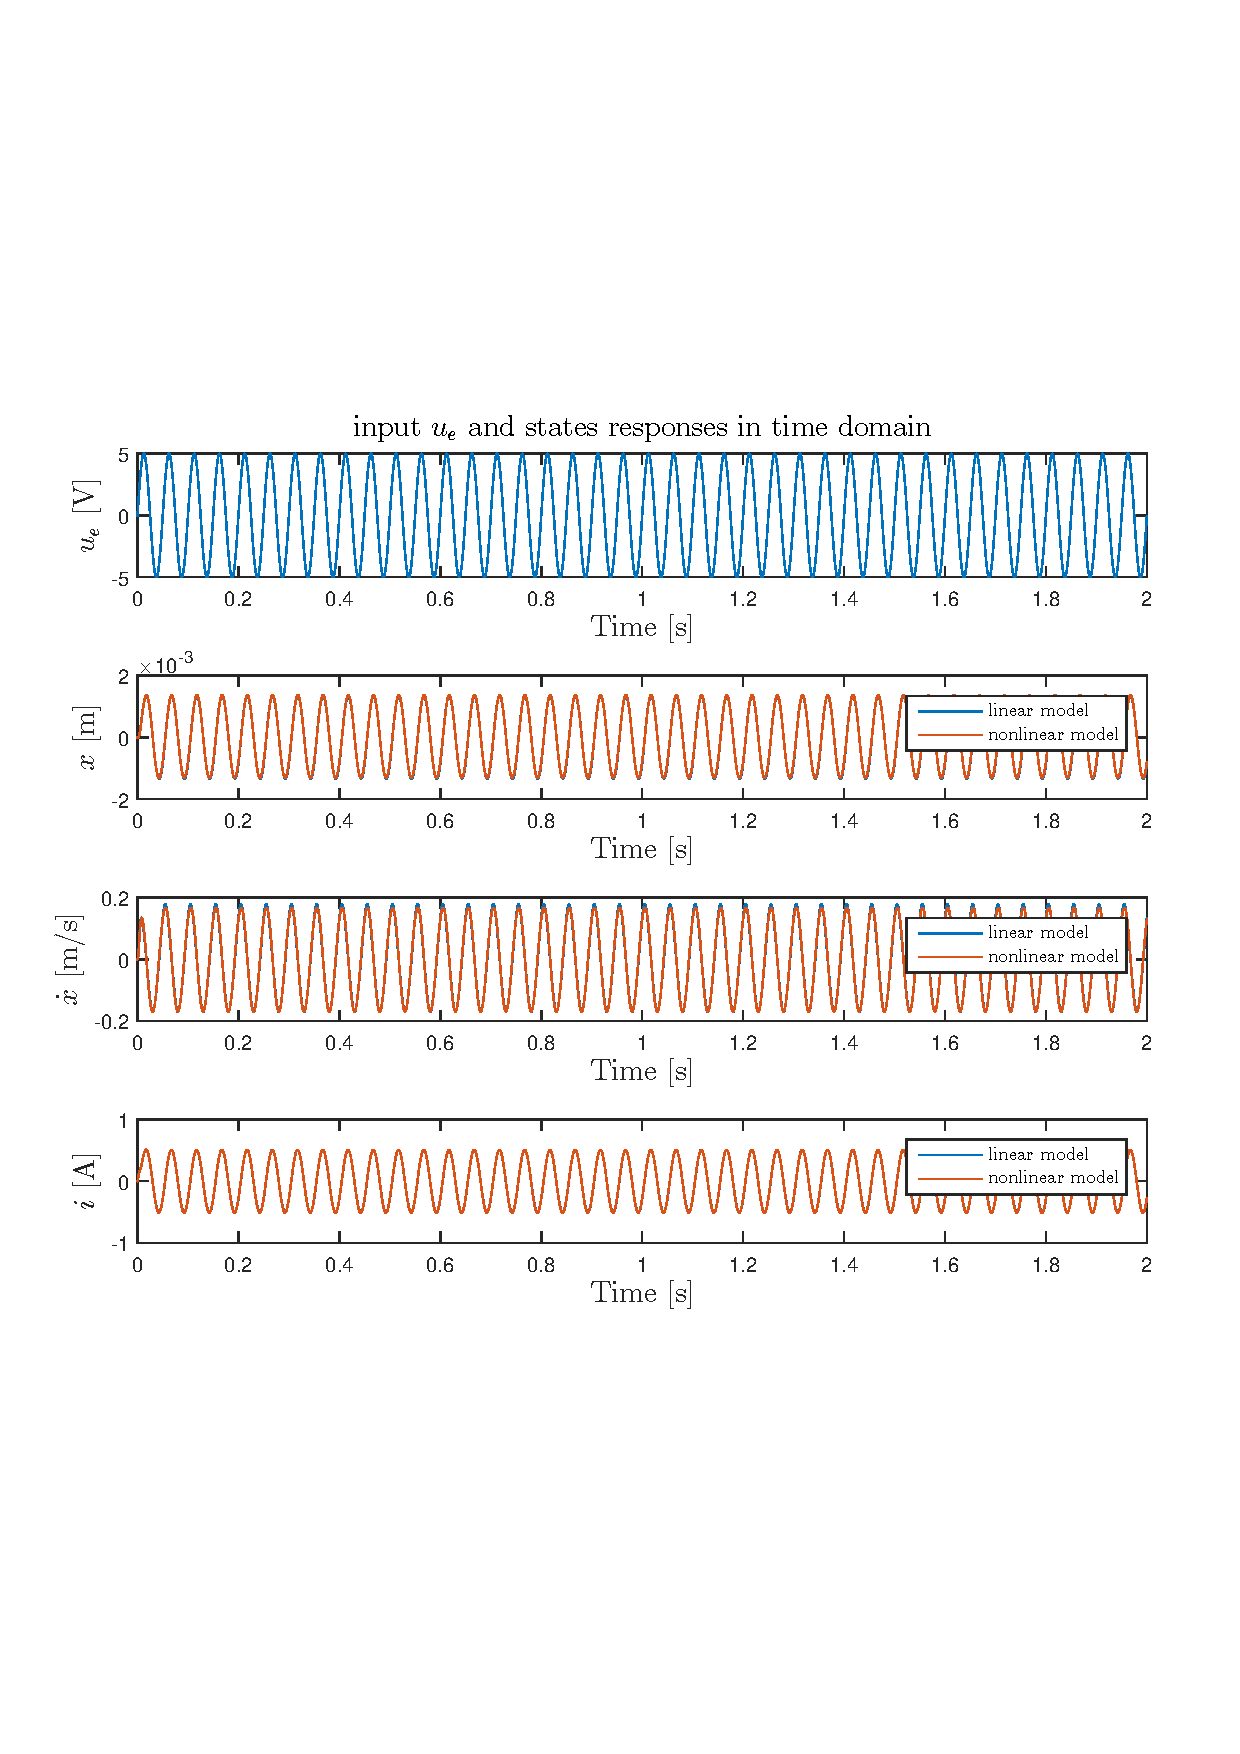
\includegraphics[trim=2cm 7cm 2cm 7cm, clip=true, totalheight=0.35\textheight, angle=0]{figures/p11time.pdf}
 \caption{response of the states to the input $u_e$ using the linearised model extended with disturbances and the nonlinear model}
 \label{fig:responseNoiset}
\end{figure}

\begin{figure}[H]
 \centering 
 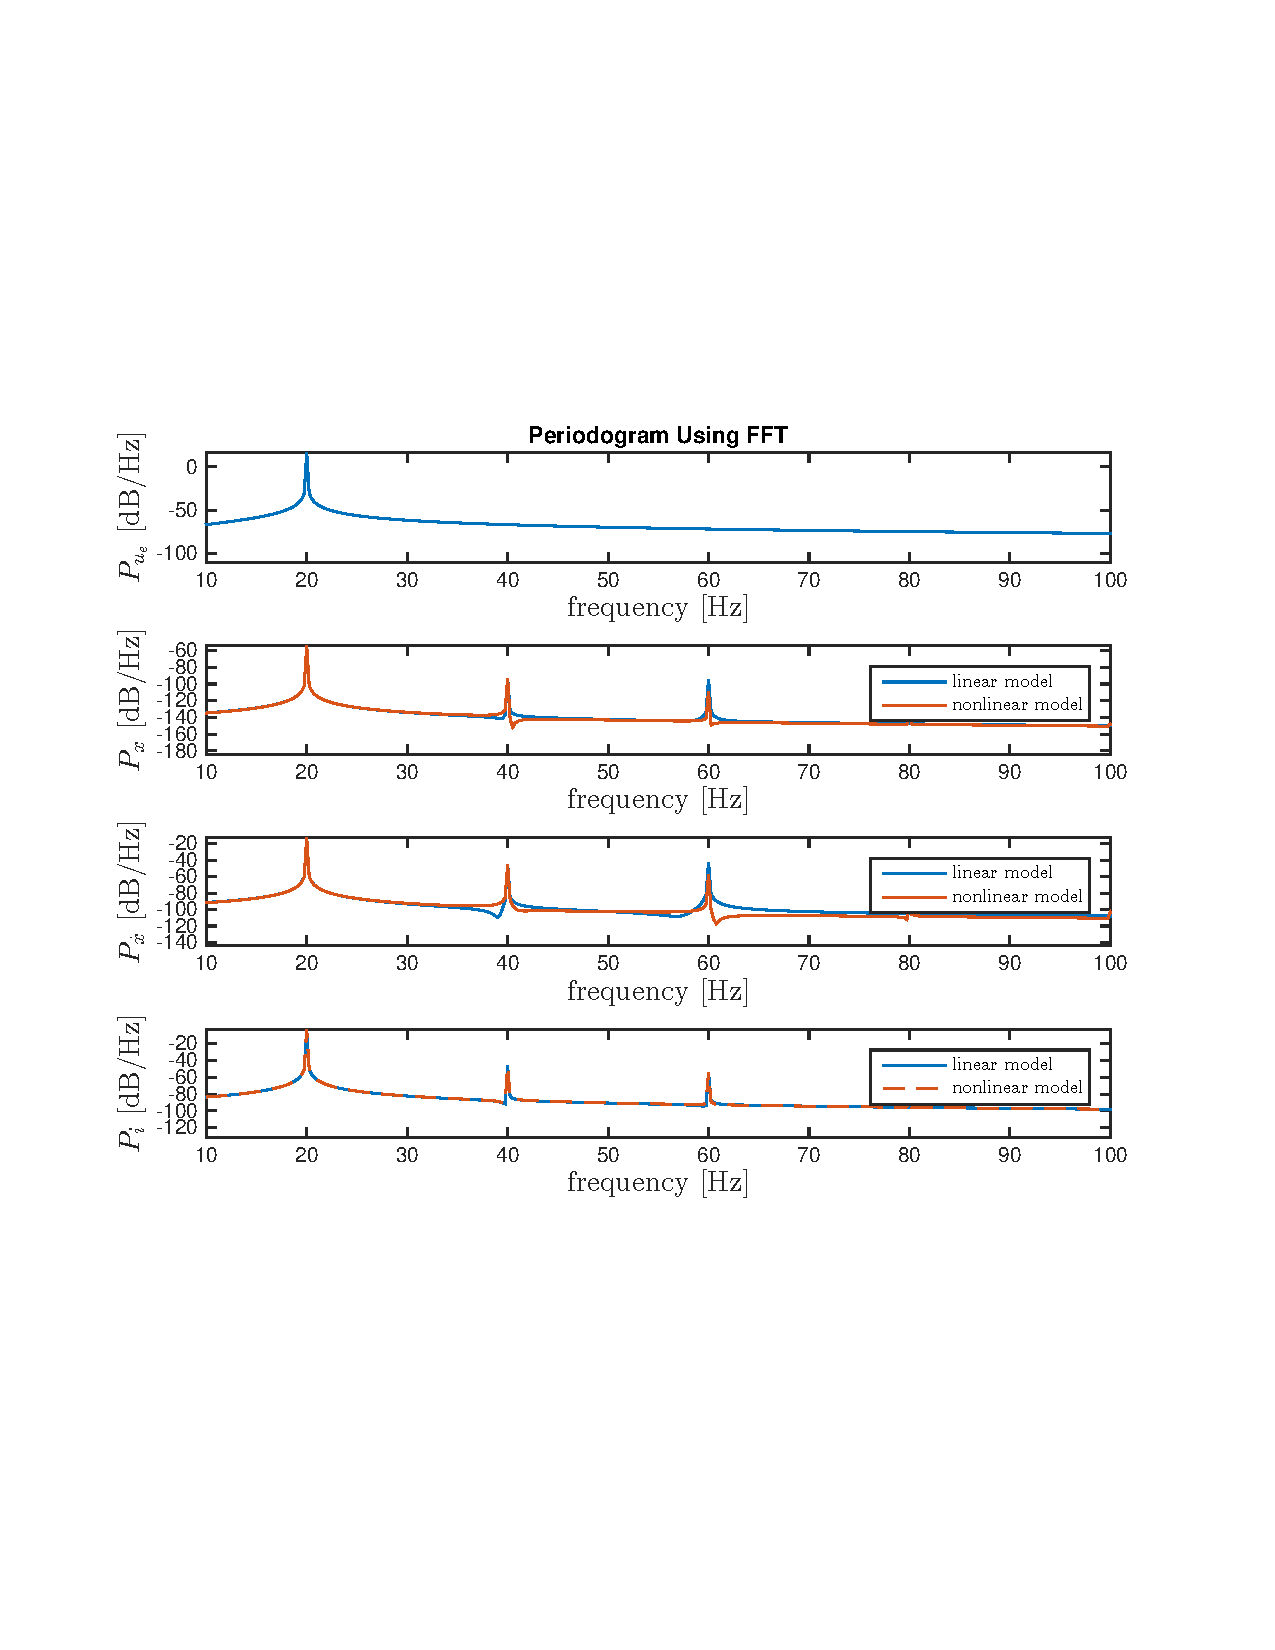
\includegraphics[trim=2cm 7cm 2cm 7cm, clip=true, totalheight=0.35\textheight, angle=0]{figures/p11freq.pdf}
 \caption{PSD of the states using the linearised model extended with disturbances and the nonlinear model}
 \label{fig:responseNoisef}
\end{figure}

We can see on both figures (\ref{fig:responseNoiset} and \ref{fig:responseNoisef}) that the responses are almost exactly the same (the plot of the response of the nonlinear model is over the one of the linear model). As expected, the two harmonic distortions of $40$ and $60$ $Hz$ are present with the right magnitude. The next distortions are of course missing. Also, the magnitude of the harmonics of state $i$ are almost perfect, but not the ones of the other states which is normal because the disturbance is designed for $i$.

